% !TEX root = ../stellar-notes.tex

\DefineShortVerb{\|}

\begin{mesaproject}[A contracting pre-main-sequence star]
\label{m.MESA-contraction}

\subsection{Setting up your workspace}

To install \mesa\ on your personal linux or mac computer do the following.
\begin{enumerate}
	\item Download and install the appropriate SDK, available from \url{http://www.astro.wisc.edu/~townsend/static.php?ref=mesasdk}. 
	\item Use \code{svn} to checkout the latest release verion of \MESA. Instructions are available from \url{http://mesa.sourceforge.net}.
	\item From a terminal window, go into the top-level \mesa\ directory and execute the following command: `|./install|'.  This may take some time as \mesa\ will be building fairly large datasets for the equation of state and opacity.  If all goes well, you will get a message at the end indicating that \mesa\ installation was successful. For a full list of instructions, see the documentation at \url{https://docs.mesastar.org/en/latest/index.html}.
\end{enumerate}

Once you have \mesa\ installed, you then set up your work environment. To do this, you create a project directory and set environment variables so that your \code{FORTRAN} compilers can find the \mesa\ libraries.

\subsection{Running your first MESA project}

You are now ready to compile and run your first \mesa\ project for this course. This is a model of a $\val{1}{\Msun}$ pre-main-sequence star. The code stops when the luminosity from hydrogen fusion first exceeds 0.95 of the luminosity from the surface. 

Download the folder |1M-pms| and place it into your projects folder.

Now execute `|./mk|'. This will call the fortran compiler to build the executable. 

If everything compiles okay, then an executable file called `|star|' will be placed in the directory. To run \mesa, type `|./rn|' at the prompt.  If all goes well, after some time a window should appear with an animated plot looking something like Figure~\ref{f.mesa-fig}. Note that during the first 300 steps of the run, \mesa\ is relaxing an initial guess for the stellar structure into hydrostatic equilibrium. After that the star is allowed to start contracting, and it quickly settles into a fully convective, contracting, pre-main-sequence star.

\begin{figure}[htbp]
\centering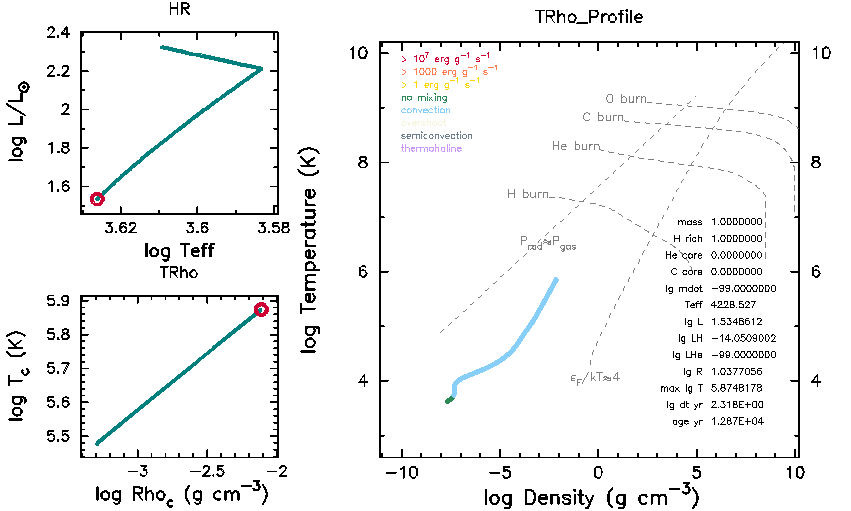
\includegraphics[width=0.9\textwidth]{Grid1_00240}
\caption{Graphical output from a \mesa\ run of a $\val{1}{\Msun}$ PMS star. \label{f.mesa-fig}}
\end{figure}

The large plot labeled `|TRho_profile|' shows the run of temperature $T$ versus density $\rho$ in the star, with the various colors indicating mixing and energy generating regions. The small plot labeled `|HR|' traces the history of luminosity $L$, in units of the solar luminosity $\Lsun$, versus effective temperature $\Teff$. The other small plot labeled `|TRho|' traces the history of the central temperature $T_{c}$ versus the central density $\rho_{c}$.

\begin{exercisebox}[Contraction of a star to the main sequence]
\begin{enumerate}
\item How long did the star take to contract to the main sequence?
\item What are $L$, $\Teff$, $T_{c}$, and $\rho_{c}$ when the star begins H burning?
\item Describe how the fraction of the star that is convective changes during the run.
\end{enumerate}
\end{exercisebox}

\subsection{A peak under the hood}
To understand what just happened, we start with the command `|./rn|'. This is just a script---you can open it with a text editor---containing the following.
\VerbatimInput{introduction/1M-pms/rn}
This just gets some information about the version of \mesa\ being used (the `|svn info|' directive), removes any pre-existing file with restart information, prints the date, runs star, and then prints the date again.

The command `|star|' is built from the source code in `|src/run.f90|'. This is a very short program.  The relevant lines
\VerbatimInput[firstline=11,lastline=16]{introduction/1M-pms/src/run.f90}
direct the program to read in parameters from a file `|inlist|' and then hand control to a subroutine, `|do_run_star|', within the \mesa\ library.

The file `|inlist|', is divided into five sections (each section begins with an `|&|' followed by the section name and ends with a `|/|'): `|star_job|', `|eos|', `|kap|', `|controls|', and `|pgstar|'.  The bang `|!|' denotes the start of a comment. This list is rather simple. The first section
\VerbatimInput[firstline=7,lastline=12]{introduction/1M-pms/inlist}
tells \mesa\ to read another file, `|inlist_1M_pms|'. Sections 2--4, `|&eos|', `|&kap|', and `|&controls|', are similar and also tell \mesa\ to read in `|inlist_1M_pms|'. It is in `|inlist_1M_pms|' that all of the non-default settings are placed.

The third section of `|inlist|'
\VerbatimInput[firstline=39,lastline=47]{introduction/1M-pms/inlist}
reads in the parameters for the plot from `|inlist_pgstar|'. There is another parameter file, `|inlist_track_central_vars|', but the flag to read that file is 
`|read_extra_pgstar_inlist2 = .false.|'  As you might guess, you'll be using this later on in the assignment.

\begin{center}
\fbox{\parbox{0.96\textwidth}{\textbf{Question:} There is a reason for nesting the parameter inlist files. Can you discern what that reason is?}}
\end{center}

In |inlist_1M_pms|', within section `|&star_job|', the lines
\VerbatimInput[firstline=12,lastline=13]{introduction/1M-pms/inlist_1M_pms}
triggers \mesa\ to start with initial star with too low a central temperature to begin hydrogen fusion, and to let that model contract. The next set of instructions
\VerbatimInput[firstline=15,lastline=19]{introduction/1M-pms/inlist_1M_pms}
tells \mesa\ not to save a \newterm{model}\sidenote{A model refers to a snapshot of the star at a given time. The saved file can be used to start a new \mesa\ run.} when it finishes, but to save model number 100. When \mesa\ constructs a pre-main-sequence model, the first steps (default is the first 300) are used to relax the star into hydrostatic equilibrium; and then the model numbers reset. By setting |save_model_number = 100|, we are asking \mesa\ to save the state of the star 100 timesteps after this initial relaxation. The model 100 is saved in the file `|1M_PMS.mod|', which we will use in subsequent exercises. The next set of lines
\VerbatimInput[firstline=21,lastline=24]{introduction/1M-pms/inlist_1M_pms}
tell \mesa\ to pause and wait for the user to hit `|return|' before ending the run, and to activate the graphical output. 

In section `|&controls|' of `|inlist_1M_pms|', the lines
\VerbatimInput[firstline=49,lastline=50]{introduction/1M-pms/inlist_1M_pms}
tell \mesa\ the initial mass and metallicity of the star, while the lines
\VerbatimInput[firstline=53,lastline=54]{introduction/1M-pms/inlist_1M_pms}
tell \mesa\ to stop when the total power from nuclear burning, $L_{\mathrm{nuc}}$, exceeds $0.95 L$, where $L$ is the total surface luminosity.

Now that you've seen the code in action, we are going to look a bit more at the architecture of \mesa. If you do `|ls $MESA_DIR|', you will see that \mesa\ is divided into modules: `|eos|' computes the equation of state, `|kap|' computes the opacity, and so forth. Within each module are two folders, `|public|' and `|private|'.  The `|public|' folder contains the interface of that module. The source file ending with `|_def.f90|' contains the data structures used by that module, and the source file ending with `|_lib.f90|' contains the routines for that module. The |private| directory contains the inner machinery of the module.

While all of these modules can be used by themselves, the `|star|' module puts everything together to simulate stellar evolution. What |star| does is to evolve a stellar model---a complete description of a star at a given instant of time---forward in time by some amount $\Delta t$. String together a sequence of such models and you have a representation of the star's evolution. These models are not evenly spaced in time; rather, \mesa\ adjusts $\Delta t$ to keep the models accurate within specified tolerances. The |star| module contains, in addition to the |public| interface and |private| machinery, additional routines in the folder |job| for starting a run from some initial model and stopping that run when a specified condition is met.

\subsection{A MESA project}

The \mesa\ code that you installed is a library, a collection of routines that when combined simulate the evolution of a stellar-like object. To put everything together, you create a directory, such as `|1M-pms|'.  A template for such a directory is contained in `|$MESA_DIR/star/work|'---consult the `|README.rst|' file there for instructions. 

The working directory is organized into several sub-directories. The `|make|' folder contains the `|makefile|' script for compiling the code. The `|src|' folder contains, in addition to the top-level `|run.f90|' code, a collection of customizable routines in the file `|run_star_extras.f90|'. In addition to these folders, the working directory contains a set of inlist files; these, as mentioned above, contain all of the parameters necessary to control the \mesa\ run and its output.  The complete listings of parameters and their default settings are contained in the directory `|$MESA_DIR/star/defaults|' in the three files `|*.defaults|'. The inlists in the work directory only need to contain those parameters that differ from the defaults.

The final components of the working directory are sub-directories to hold the output of \mesa.  The names of these are customizable and can be set in the inlists; by default, the main two are called `|LOGS|' and `|photos|'.  Within `|LOGS|' are the file `|history.data|' and the files `|profile|\textit{dd}|.data|'. The `|history.data|' file contains the time evolution of global stellar properties, such as luminosity, radius, surface effective temperature, and so on. The `|profile|\textit{dd}|.data|' files contain ``snapshots'' of the star's structure: the run of temperature, density, pressure, and so on with location within the star. 

\subsection{Exercise: customizing MESA output}

After that brief overview of the \mesa\ architecture, let's do something concrete: we shall customize \mesa\ to have it generate a plot of a variable that we define.  In this chapter, we've argued that the central pressure of a star should scale as $P_{c}\propto GM^{2}/R^{4}$. We also found that the central density should scale as the mean density, $\rho_{c}\propto \bar{\rho} = 3M/(4\pi R^{3})$. Exercise~\ref{ex.central-temperature} asks you to find the central temperature in terms of $M$, $R$, and mean molecular weight $\mu$. What the derivation in the chapter doesn't tell us is the coefficient $\rho_{c}/\bar{\rho}$ and its counterparts for pressure and temperature.  We can use \mesa, however, to test these scalings and extract these coefficients.

To do this, we modify the code in `|src/run_star_extras.f90|'.  What we want is for \mesa\ to calculate $P_{\mathrm{scale}} = GM^{2}/R^{4}$, $\rho_{\mathrm{scale}} = \bar{\rho}$, and $T_{\mathrm{scale}}$, and then write out the values of $P_{c}/P_{\mathrm{scale}}$, $\rho_{c}/\rho_{\mathrm{scale}}$, and $T_{c}/T_{\mathrm{scale}}$ in the file `|history.data|'. To do this, we first tell \mesa\ how many extra columns in `|history.data|' we need:
\VerbatimInput[firstline=121,lastline=129,gobble=8]{introduction/1M-pms/src/run_star_extras.f90}
Here I am adding one column, which will be $P_{c}/P_{\mathrm{scale}}$.  When you implement the other scalings, you'll change the variable \verb|how_many_extra_history_columns| to reflect that we need three columns.

Next, we need to compute the data for these columns.  We therefore modify the following routine.
\VerbatimInput[firstline=132,lastline=175,gobble=8]{introduction/1M-pms/src/run_star_extras.f90}
In detail, we first declare the extra variables we need.
\VerbatimInput[firstline=138,lastline=138,gobble=8]{introduction/1M-pms/src/run_star_extras.f90}
Next, we give each column a name.
\VerbatimInput[firstline=147,lastline=149,gobble=8]{introduction/1M-pms/src/run_star_extras.f90}
Notice that the latter two are commented out (`|!|'); for this example; you'll need to uncomment them to print out the other variables.

We are then ready to compute our values. Note that \mesa\ defines many physical constants in `|$MESA_DIR/const/public/const_def.f90|', so we should use those values.  For example, we load the value of Newton's gravitational constant in line 153, and you can read the hint in lines 166ff for loading $\kB\NA$. Next, we need to get the values of $M$, $R$, $\mu_{c}$, $P_{c}$, $\rho_{c}$, and $T_{c}$. These are provided in an internal data structure, which the routine loads into a pointer named `|s|'
\VerbatimInput[firstline=141,lastline=141,gobble=8]{introduction/1M-pms/src/run_star_extras.f90}
with the data structure being tagged with the variable |id| that is passed to the routine.  To see a complete list of what is in this data structure, look at `|$MESA_DIR/star_data/public/star_data.inc|'. I've already taken care of computing $M$, $R$, $\mu_{c}$, and $P_{\mathrm{scale}}$ for you. For example,
\VerbatimInput[firstline=159,lastline=159,gobble=8]{introduction/1M-pms/src/run_star_extras.f90}
takes the stored variable `|log_surface_radius|', which is $\log_{10}(R/\Rsun)$, according to `|$MESA_DIR/star_data/public/star_data.inc|'; it then uses the `|exp10|' intrinsic and the value of $\Rsun$---which is defined in `|const_def.f90|'---to get the surface radius in cgs. Finally, the characteristic pressure scaling is computed
\VerbatimInput[firstline=163,lastline=163,gobble=8]{introduction/1M-pms/src/run_star_extras.f90}
and this is used to scale the pressure and store it in the array `|vals|':
\VerbatimInput[firstline=171,lastline=171,gobble=8]{introduction/1M-pms/src/run_star_extras.f90}
You will fill in the second and third members of the array for the scaled central density and temperature.

If you look in `|LOGS/history.data|', you should see that the last column is indeed `|Pc_scaled|', as expected. Of course, we'd like to display it graphically, and \mesa\ does predefine plots that can display values in `|history.data|'. We customized the output in `|inlist_track_central_vars|':
\VerbatimInput{introduction/1M-pms/inlist_track_central_vars}
To use this, we activate the window by setting the flag in line 3 to `|.true.|', and we set `|read_extra_pgstar_inlist2 = .true.|' in the top-level inlist. If we want to save our output, we can set `|History_Panels2_file_flag = .true.|' in `|inlist_track_central_vars|'. We'll need to have the directory `|frames|` created (see line 12) to hold these. For a history plot, the default x-axis is the model number of the star. You can change this, for example, by uncommenting the line 
\VerbatimInput[firstline=15,lastline=15]{introduction/1M-pms/inlist_track_central_vars}
in `|inlist_track_central_vars|'. Finally, to plot the scaled central density and temperature, you'll need to change the number of panels and declare them, lines 17--18.

\end{mesaproject}

\UndefineShortVerb{\|}
